% !TEX TS-program = pdflatexmk
\documentclass[11pt]{article}
\usepackage[margin=1in]{geometry} 
\usepackage[parfill]{parskip}% Begin paragraphs with an empty line rather than an indent
\usepackage{amsthm}
\newtheoremstyle{oldplain}
  {\topsep}   % ABOVESPACE
  {\topsep}   % BELOWSPACE
  {\itshape}  % BODYFONT
  {}       % INDENT (empty value is the same as 0pt)
  {\bfseries} % HEADFONT
  {.}         % HEADPUNCT
  {5pt plus 1pt minus 1pt} % HEADSPACE
  {}          % CUSTOM-HEAD-SPEC
\theoremstyle{oldplain}
\newtheorem{oldthm}{Theorem}[section]
\theoremstyle{plain}
\newtheorem{thm}{Theorem}[section]  
\usepackage{graphicx}
\usepackage{url}
%SetFonts
% newpx text and math
\linespread{1.05}
\usepackage[largesc,theoremfont]{newpxtext}
\usepackage{textcomp}
\usepackage{newpxmath}
\usepackage{bm}
\useosf
%SetFonts
\usepackage{upquote}
\font\pcf=zpl-Regular-osf-sc-t1 at 10.95pt
\usepackage{booktabs}\title{New PX font package}
\author{Michael Sharpe}
\date{\today}  % Activate to display a given date or no date

\begin{document}
\maketitle
\section{Introduction}
This package is meant to be  a replacement for Young Ryu's {\tt pxfonts}---a complete text and math package with roman text font provided by a Palatino clone, sans serif based on a \textsf{Helvetica} clone, typewriter faces, plus math symbol fonts whose math italic letters are from a Palatino Italic clone. As with the related {\tt txfonts} (though not as severe) the math metrics in {\tt pxfonts} are overly tight.

The goal of this new project is use his glyphs along with a few additions and with completely reworked metrics which are generally looser, but not as loose as Computer Modern math. The following small examples (double normal size) provide some idea of the  extent of the changes.


\begin{minipage}{3.1in}
\begin{center}
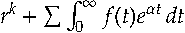
\includegraphics[scale=2]{pxfontseg-crop}\\
Math rendered with pxfonts
\end{center}
\end{minipage}
\begin{minipage}{3.1in}
\begin{center}
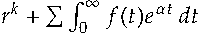
\includegraphics[scale=2]{newpxeg-crop}\\
Math rendered with newpxmath
\end{center}

\end{minipage}


This new package differs from {\tt pxfonts} in the following ways:
\begin{itemize}
\item
the new package is split into separate text and math packages that do not need to be used in conjunction;
\item both text and math packages offer options not present in the original package, described below;\item wide accent glyphs have been corrected (they should have zero depth) so that they no longer collide with the underlying glyph;
\item the summation and product symbols in {\tt pxfonts} seemed overly heavy at display size, and have been replaced by others of more suitable weights;
\item for those who do not like the integral in \textsf{pxfonts}, an emboldened version of the Computer Modern integral is made available, matching the weight of the \textsf{pxfonts} symbols;
\item an upright partial derivative symbol has been added, named \verb|\uppartial|---$\uppartial$;
\item there is now an option to get braces more pleasing to older eyes;
\item macros have been added to bring the calls to Greek symbols more into conformity with \textsc{psnfss} and Mathtime Pro~2;
\item an upright Greek \verb|\upvarkappa|, $\upvarkappa$, has been added as well as a matching italic version $\varkappa$;
\item problems using \textsc{ams} macro packages before \textsf{pxfonts} are settled;
\item \verb|\coloneq| and \verb|\eqcolon| now point to the correct glyphs;
\item The problem with the {\tt ogonek} accent  and tabular environments (bad definition of \verb|\k|) is fixed;
\item The default encoding for \textsf{newpxtext} is now T$1$, but support is offered also for OT$1$ and LY$1$. As some add-on packages are available only in T$1$, that seems the best current choice.
\item The font collection used for rendering text is based on TeXGyrePagella with a number of additions, denoted by TeXGyrePagellaX. The superior figures in this addition are set by default to render footnote markers. (It is also possible customize footnote markers by redefining \verb|\thefootnote| after loading {\tt newpxtext.sty}.) Small caps are available in all weights and styles, and are offered in two sizes. The default small caps supplied by TeXGyrePagella are really \textsc{Petite Caps}, having xheights approximately the same x-heights (sometimes smaller) than lowercase letters. Option \texttt{largesc} increases the size of small caps by about 8\%, approximating the size of Adobe Palatino Small Caps. IMO, this is a better match in terms of weight and size. For a side by side comparison: {\pcf Petite Caps}, \textsc{Small Caps}.
\item Sans serif is by default taken from TeXGyreHeros, and by default at 94\% of the scale factor (set by {\tt scaled}, default value {\tt1}). The option {\tt helvratio=.98} will change that to 98\%.
\item New math accents such as \verb|\widearc| have been introduced in tandem with the {\tt newtx} package, where they are documented.
\end{itemize}
\section{Text mode options and macros}
The text mode environment invoked by
\begin{verbatim}
\usepackage{newpxtext}
\end{verbatim}
has several options: you may write
\begin{verbatim}
\usepackage[scaled=.95]{newpxtext}
\end{verbatim}
to load the roman and typewriter text fonts at 95\% of normal size, and the sans serif (\textsf{Helvetica} clone) at scale $0.95*0.94$. This is not of much utility if the package is used with the math package {\tt newpxmath} to which it is already matched, but may be with other math packages. The options
\begin{verbatim}
\usepackage[scaled=.95,helvratio=.96]{newpxtext}
\end{verbatim}
load roman and typewriter text fonts at 95\% of normal size, and the sans serif (\textsf{Helvetica} clone) at scale $0.95*0.96$.

The option \texttt{osf} instructs the text fonts to use old-style figures \oldstylenums{1234567890} rather than the default lining figures $1234567890$. As of version $1.23$, {\tt newpxtext} loads initially with lining figures so the math package uses lining figures in math mode. The option {\tt osf} switches to old-style figures in text at the very end of the preamble, forcing the use of oldstyle figures in text, but not math. In previous versions, it was necessary to run 
\verb|\useosf| after loading math. This is no longer required unless the {\tt babel} package is loaded, but does no harm. See the discussion in section 4 for further details.



As described above, option {\tt largesc} increases the size of small caps by about 8\%.

Option {\tt defaultsups} (same effect as {\tt defaultsups=true}) forces the package to use the \LaTeX\ default footnote markers (or, at least, those in force when the package is loaded) instead of preferred by the package---Palatino (clone) superior figures instead of spindly ordinary Palatino lining figures reduced to about 70\%. (Footnote markers in minipages use the default lowercase alphabetic characters, unless otherwise specified by redefining \verb|\thempfootnote|.) For better control over position and size of footnote markers, use the {\tt superiors} package after loading {\tt newpxtext}. 

The {\tt theoremfont} option changes the default font used for the {\tt plain} theorem style of {\tt amsthm}, keeping italic text but substituting upright figures and punctuation. For example, with this option, you get theorem statements like this:

\begin{thm}
This is Theorem Italic: text numbers are upright---12345; punctuation is in many cases upright (also, parens, braces \{\} and brackets []). What about question marks and exclamations? Also upright! [These fit better with math mode punctuation and figures, like: for all $x\in[0,1]$, let $f(x)\coloneq \exp(\alpha x)$].
\end{thm}
Compare this to traditional {\tt plain} theorem style of the same text:
\begin{oldthm}
This is Theorem Italic: text numbers are upright---12345; punctuation is in many cases upright (also, parens, braces \{\} and brackets []). What about question marks and exclamations? Also upright! [These fit better with math mode punctuation and figures, like: for all $x\in[0,1]$, let $f(x)\coloneq \exp(\alpha x)$].
\end{oldthm}


Superior letters and figures may be called with either \verb|{\sustyle ...}| or \verb|\textsu{...}|, so you can emulate $18$\textsu{th} century orthography such as J\textsu{os} W\textsu{m} Smith, or print French style with , e.g., $1$\textsu{i\`ere}, M\textsu{me} Dubois or M\textsu{lle} D'Orleans.

The next two sections describe options to {\tt newpxtext} of more specialized nature.

\section{Spacing issues}
This new version of {\tt newpxtext} has spacing that is a little different, in its default state, from that of the old {\tt newpxtext}. In small part this is due to the finer kerning of TeXGyre Pagella, but mostly because the three parameters that govern inter-word spacing are not the same.
\begin{verbatim}
                               pxfonts     Pagella
fontdimen2 (interword space)   .25em       .25em
fontdimen3 (interword stretch) .125em      .2em
fontdimen4 (interword shrink)  .08333em    .1em
\end{verbatim}
That is, {\tt Pagella} has the same normal spacing as {\tt pxfonts} but its spacing is more flexible in terms of both stretch and shrink. More frequently than not, a paragraph built with {\tt Pagella} will occupy more space than the same built with {\tt pxfonts}. For this reason, the package offers some ways to change the spacing parameters. This may be important if you are trying to imitate the pagination of a document built using~{\tt pxfonts}.

Option {\tt tighter} sets the three fontdimen values to those of {\tt pxfonts}, except with a little more shrink. This should make it unlikely that text will occupy more space than it would have using~{\tt pxfonts}. 

Option {\tt looser} sets the three fontdimen values to \verb|{.3em,.2em,.1em}| respectively. 

If you want full control, the options {\tt spacing, stretch, shrink} allow you to modify one or more of the above fontdimens. For example,
\begin{verbatim}
\usepackage[stretch=.15em,shrink=.095em]{newpxtext}
\end{verbatim}



\section{Usage with {\tt babel}}
You should normally load {\tt babel} before loading {\tt newpxtext} in order for {\tt babel} to function as expected. {\tt Newpxtext} will set an internal flag to indicate that {\tt babel} is being used. Option \texttt{babel} should be used only if you are forced to load {\tt babel} after {\tt newpxtext}. There appears  to be  an incompatibility between parts of {\tt babel} and \verb|\AtEndPreamble|. If you use {\tt babel}, and a math package, you have to omit the {\tt osf} option and use the macro \verb|\useosf| after loading the math package if you want oldstyle figures in text mode and lining figures in math mode. A similar macro \verb|\useproportional| makes proportional figures the deafault outside math mode. For example:
\begin{verbatim}
\usepackage[greek.polutonico,english]{babel}
\usepackage[theoremfont,largesc,tighter]{newpxtext}
\usepackage[T1]{fontenc}
\usepackage{textcomp}
\usepackage[varqu,varl]{inconsolata}
\usepackage{amsmath,amsthm}
\usepackage[bigdelims,vvarbb]{newpxmath}
% option vvarbb gives you stix blackboard bold
\useosf
\useproportional 
\linespread{1.05}
\end{verbatim}


\section{Math mode options}
The package invoked by
\begin{verbatim}
\usepackage{newpxmath}
\end{verbatim}
loads the math part of the {\tt pxfonts} (with revised metrics and additional glyphs) and should be loaded \emph{after} the text font and its encoding have been specified, as it uses the text font settings to define how operators, numbers, math accents, \verb|\mathrm|, \verb|\mathbf| etc.\ are rendered. You should also load a Typewriter font so as not to generate mysterious error messages about \textsf{metafont} trying to generate \texttt{ectt10}. The package offers a number of options.
\begin{itemize}
\item 
\begin{itemize}
\item{\tt varg} causes the math italic letter $g$ to be replaced by $\varg$;
\item{\tt cmintegrals} instructs \textsf{newpxmath} to load a thicker version of the Computer Modern integral in place of the \textsf{newpxmath} default---the pxfonts integral (identical to the integral in the Wolfram fonts), which is not to everyone's taste---a consequence is that none of the special forms of \textsf{pxfonts} integrals are available;
\item The option {\tt cmbraces} instructs {\tt newpxmath} to ignore the brace collections from {\tt pxfonts}, substituting a collection based on thickened versions of the Computer Modern braces, which I find much easier to distinguish from other delimiters. This works quite well in regular weight but looks a bit clunky in bold.
\item [NEW] The new option {\tt bigdelims} offers delimiters which are a bit larger than the standard delimiters and the normal and {\tt big} sizes, with more distinction between the two than in the standard package. With {\tt bigdelims}, the option {\tt cmbraces} is ignored.
\end{itemize}
\item the combination
\begin{verbatim}
\usepackage{amsmath}% loads amstext, amsbsy, amsopn but not amssymb
\usepackage{newpxmath}
\end{verbatim}
causes no error, unlike the same combination with {\tt pxfonts}, but does nothing significant. The package {\tt newpxmath} loads the package {\tt amsmath} if it was not previously loaded. Options to {\tt amsmath} such as {\tt leqno,intlimits} may be passed to {\tt amsmath} via options to the documentclass. The integrals are as defined in {\tt pxfonts}. With
\begin{verbatim}
\usepackage[cmintegrals]{newpxmath}
\end{verbatim}
you may use the forms \verb|\iint|, \verb|\iiint|, \verb|\iiiint| and \verb|\idotsint| defined in {\tt amsmath}, but using the pumped-up Computer Modern integral loaded by {\tt newpxmath}. 
\item {\tt uprightGreek} and {\tt slantedGreek} determine the form of Greek alphabet loaded---the default is {\tt uprightGreek}, which loads upright uppercase and slanted lowercase Greek symbols, as is customary in Anglo-American mathematical typesetting. With the option {\tt slantedGreek}, which you might want to use if you cared about ISO standards, all Greek symbols are slanted. No matter which is set, \verb|\Gammaup| (or \verb|\upGamma|) gives you upright \verb|\Gamma|, etc.
\item The \textsf{newpxmath} package contains three different Blackboard Bold alphabets, where original \textsf{pxfonts} contained one. The default, triggered by \verb|\mathbb{}|, takes its glyphs from the font which replaces {\tt msbm} and has the same overall appearance of a hollowed-out text font, which I find neither bold nor blackboard-like. The second option, taken from \textsf{pxfonts}, is triggered by \verb|\varmathbb{}|, is more geometric and, in my opinion, preferable but not optimal. The option {\tt varbb} makes \verb|\mathbb{}| synonymous with \verb|\varmathbb{}|. The third option is the double-struck glyphs from the STIX collection. See the expanded discussion below.
\item {\tt nosymbolsc} causes the package to not load the {\tt symbolsC} fonts, saving  a math family. (This font contains mostly exotic symbols, along with some very useful, commonly used symbols like \verb|\coloneq| $\coloneq$, \verb|\eqcolon| $\eqcolon$, \verb|\notin| $\notin$, \verb|\notni| $\notni$, \verb|\neq| $\neq$, \verb|\nsubset| $\nsubset$ and \verb|\nsupset| $\nsupset$, but these have been moved (virtually) to {\tt lettersA} so they may continue to be used even if you use the option {\tt nosymbolsc}.)
\item {\tt amssymbols} (the default) and {\tt noamssymbols} determine whether the {\tt pxfonts} versions of the \textsc{ams} symbols ({\tt msam}, {\tt msbm}) are loaded---if so, they override previous settings in {\tt amsmath}. If you use the option {\tt noamssymbols}, then \verb|\mathbb{}| is set to mean the same as \verb|\varmathbb{}|. (One advantage of {\tt noamssymbols} is that you save two of your precious math families for other purposes, such as setting a couple of external math alphabets by means of the \textsf{mathalfa} package.)
\end{itemize}

\textsc{Example:}
\begin{verbatim}
\documentclass[leqno]{article}
\usepackage[osf,theoremfont]{newpxtext} % T1, lining figures in math, osf in text
\usepackage{textcomp} % required for special glyphs
\usepackage[varg,cmintegrals,bigdelims]{newpxmath}
\usepackage[scr=rsfso]{mathalfa}% \mathscr is fancier than \mathcal
\usepackage{bm} % load after all math to give access to bold math
%\useosf %no longer needed unless using babel
\linespread{1.05}% Give Palatino more leading (space between lines)
\end{verbatim}

\textbf{Caution:} In encodings {\tt T1} and {\tt LY1}, the macro \verb|\mathrm| does not produce what you might expect for Greek letters, due to the difference between those encodings and {\tt OT1}. But what were you expecting with \verb|\mathrm{Gamma}| anyway? In {\tt T1} and {\tt LY1}, you'll get a math accent.

\section{The \TeX\ math font problem}
Math font packages in \LaTeX\ are susceptible to the ``Too many math alphabets'' error, due to exceeding the limit of just sixteen math font families, or mathgroups, as they are called in \LaTeX. Put in oversimplified terms that do however correctly represent how this all works in \textsf{newpxmath}, the following math fonts are always loaded and permanently (if you didn't prevent loading of some features) occupying slots immediately following \verb|\begin{document}|, and others that may be called for in typesetting a mathematical expression can add to the list as the document grows.

\textsc{Always loaded:}
\begin{verbatim}
0: operators
1: letters
2: symbols
3: largesymbols
4: AMSa
5: AMSb
6: lettersA
7: symbolsC
8: largesymbolsTXA
9: boldoperators
10: boldletters
11: boldsymbols
12: boldlargesymbols
\end{verbatim}
\textsc{Notes:}
\begin{itemize}
\item
The {\tt operators} font is essentially the Roman text font, used for names of operators and as the target for \verb|\mathrm|---its bold version is used as the target for \verb|\mathbf|;
\item if you typeset an expression that, say, calls for a single bold glyph from  {\tt symbolsC}, that costs you an entire new slot, leaving only two remaining;
\item same with, eg, \verb|\mathit|;
\item same with an external Fraktur, Blackboard Bold or Script glyphs;
\item if you run out of math alphabets, look first to dropping {\tt AMSa} and {\tt AMSb}, as well as {\tt symbolsC}, which can save you three slots;
\item if space is tight, do not call bold versions of the fonts listed above where the bold version is not already loaded, to avoid loading a new mathgroup; 
\item if you absolutely need a letter (not a math symbol) from some math font that would normally cost you another mathgroup, you might consider using as if it were text, with something like
\begin{verbatim}
\mbox{{\usefont{U}{zplmia}{b}{n} X}}
\end{verbatim}
which allows you to use letter X from {\tt boldlettersA} but without any math features;
\item there is a macro \verb|\ShowMathFonts| in {\tt newpxmath} which may be called at any point in your document, which will provide you a list of the mathgroups currently in use. This can be helpful in figuring out where problems occur. The output lines take the form
\begin{verbatim}
(<fam number>: <internal font id> = <tfm name> [newpx name])
\end{verbatim}

\end{itemize}
\section{Bold math fonts}\label{sec:boldmath}
Every math font in the {\tt pxfonts} package, and in the {\tt newpx} package, is accompanied by a bold version. Some usage examples are given below. Generally, one may use either \verb|\boldmath| to change an entire formula to bold, or \verb|\boldsymbol| to change one symbol, but the spacing generally works better after loading the {\tt bm} package and using the \verb|\bm| macro.

The text glyphs dotlessi (\verb|\i|) and dotlessj (\verb|\j|) are rarely needed in actual text---in many fonts, roman dotlessi is very similar to the numeral 1. They are however sometimes needed to build special math glyphs. The following table shows how to generate the mathematical forms of dotlessi and dotlessj. I illustrate with only dotlessi---dotlessj is entirely analogous.

\begin{center}
  \begin{tabular}{@{} llll @{}}
    \hline
    Type & Weight & Command & Result \\ 
    \hline
    Math Italic & Regular & \verb|$\hat{\imath}$| & $\hat{\imath}$ \\ 
    Math Italic & Bold & \verb|$\bm{\hat{\imath}}$| & $\bm{\hat{\imath}}$ \\ 
    Roman & Regular & \verb|$\hat{\textrm{\i}}$| & $\hat{\textrm{\i}}$\\ 
    Roman & Bold & \verb|$\bm{\hat{\textbf{\i}}}$| & $\bm{\hat{\textbf{\i}}}$\\ 
    \hline
  \end{tabular}
\end{center}
\newcommand{\xyvec}[2]{\ensuremath{#1\bm{\textbf{\i}}#2\bm{\textbf{\j}}}}

In math, bold roman characters are often used to indicate vector quantities, and for this one uses constructions like 
\begin{itemize}
\item
\verb|$\mathbf{x}$| produces $\mathbf{x}$;
\item
\verb|$\bm{\mathrm{x}}$| produces $\bm{\mathrm{x}}$ (same as previous but may offer improved spacing);
\item
\verb|$\bm{x}$| produces $\bm{x}$ (not roman);
\item
\verb|$\bm{\hat{\mathbf{x}}}$| produces $\bm{\hat{\mathbf{x}}}$ (with a bold accent);
\item \verb|$\bm{\dot{x}}$| produces $\bm{\dot{x}}$ (bold but not roman);
\item the macro definition
\begin{verbatim}
\newcommand{\xyvec}[2]{\ensuremath{#1\bm{\textbf{\i}}#2\bm{\textbf{\j}}}}
\end{verbatim}
allows you to write \verb|\xyvec{x}{+y}| to output $\xyvec{x}{+y}$;
\item \verb|$\bm{\Gamma}$| produces $\bm{\Gamma}$ (bold Gamma);
\item \verb|$\bm{\hat{\Gamma}}$| produces $\bm{\hat{\Gamma}}$ (bold Gamma with bold accent).
\end{itemize}
(The last two assume that you have effectively set the option {\tt uprightGreek}---the default.)

\section{Blackboard bold}
As mentioned briefly above, the package now has a new blackboard bold alphabet built-in, and some new macros to call the non-default versions. To summarize, the problems are:
\begin{itemize}
\item
the default, called by \verb|\mathbb| is quite ugly and indistinct, but does cooperate with the bolding macros \verb|\bm| and \verb|\boldsymbol|;
\item the original variant form called with the macro \verb|\varmathbb| is better, but the macro conflicts with \verb|\bm|. (In fact, the bold version is identical to the regular version, but it is still not right that it conflicts with them.) The problem stems from the part of the definition of \verb|\varmathbb| which allows you to insert an argument with more than one character, like \verb|\varmathbb{ABC}|. The solution is to make a new macro that takes a single argument, like \verb|\vmathbb{A}|, which cooperates with \verb|\bm|.
\item the third, new, alphabet is borrowed from the STIX fonts---it is sharp and quite clear, geometric in design. The only slight problem is that it lacks a full bold version, with only the letters C, D, H, N, P, Q, R, Z, d, e, i and j available. The macro \verb|\vvmathbb| provided to access this alphabet allows only a single character for its argument. The new option {\tt vvarbb} effectively makes \verb|\mathbb| mean the same as \verb|\vvmathbb|.
(The reason for including these in the \textsf{newpx} package rather than calling them from the \textsf{mathalfa} package is that \textsf{newpx} leaves very little space for new math symbol fonts and math alphabets, and this way requires no additional such resources.
\end{itemize}
One interesting feature of the new alphabet is that it contains blackboard bold numbers, of which $0$ and $1$ will likely be the most useful, perhaps as operator names. I find $\vvmathbb{1}$=\verb|$\vvmathbb{1}$| useful in specifying an indicator, AKA characteristic function. Here are some examples:

\begin{center}
  \begin{tabular}{@{} llll @{}}
    \toprule
     & Regular & Bold & Remarks \\ 
    \midrule
Default  & \verb|$\mathbb{R}$| $\mathbb{R}$& \verb|$\bm{\mathbb{R}}$| $\bm{\mathbb{R}}$\\ 
Variant 1     & \verb|$\varmathbb{R}$| $\varmathbb{R}$ &  & Bold is same as regular \\ 
$\dots$or     & \verb|$\vmathbb{R}$| $\vmathbb{R}$ &  & Single char.\ argument\\ 
Variant 2 & \verb|$\vvmathbb{R}}$| $\vvmathbb{R}$& \verb|{\boldmath $\vvmathbb{R}$}| {\boldmath $\vvmathbb{R}$} & Make a macro for this! \\ 
%     & $\bm{\mathbb{AB}}$  & $\bm{\vmathbb{A}\vmathbb{B}}$ & $\bm{\vvmathbb{A}\vvmathbb{B}}$ \\ 
    \bottomrule
  \end{tabular}
\end{center}


\end{document}  